\section{Wichtige Stoffe + Struktur}
\subsubsection{Kohlenhydrate}
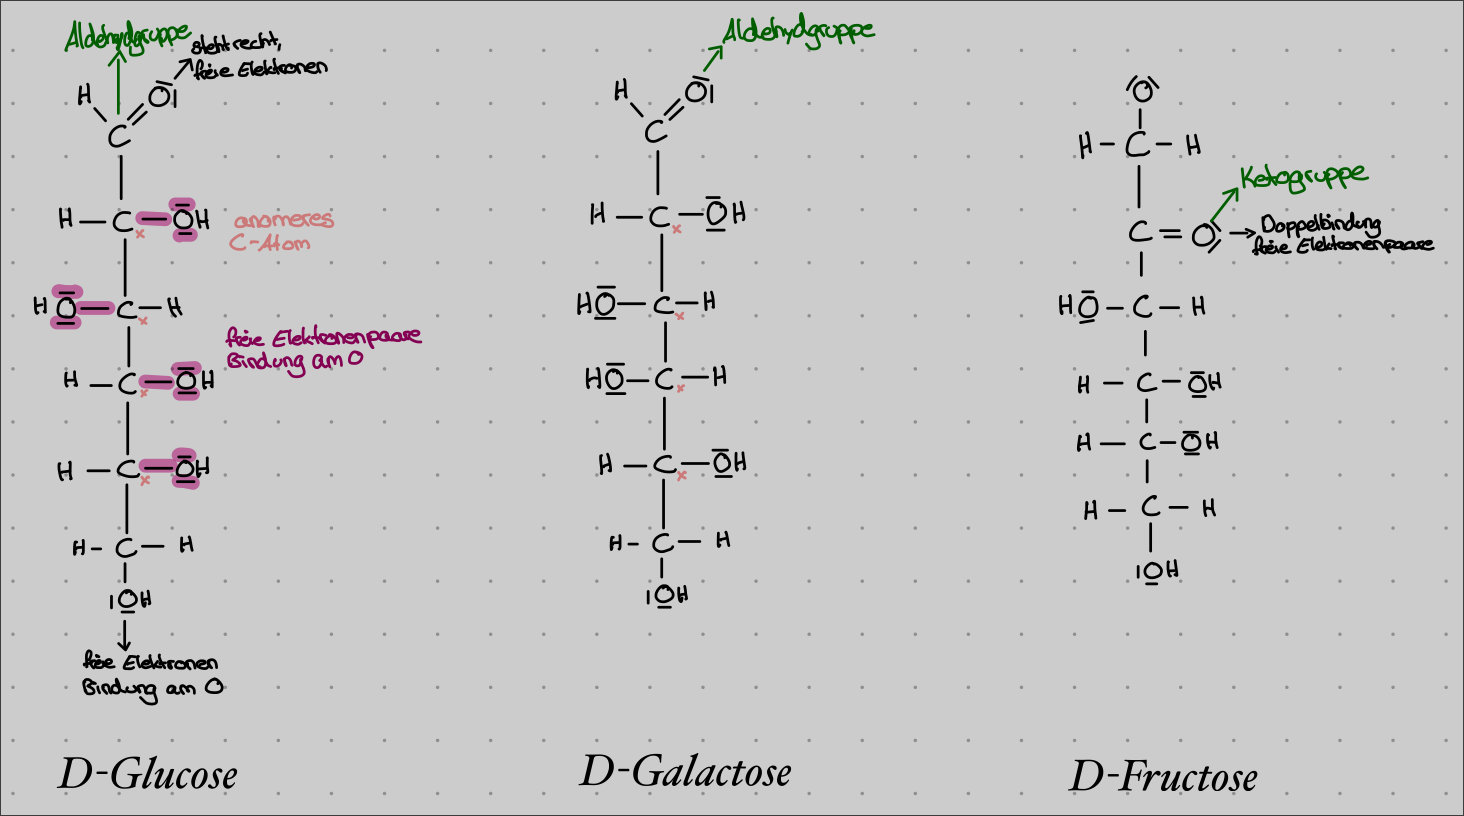
\includegraphics[scale=0.30]{media/naturstoffe/stoffe.png} \\\\
%D-Glucose: 
%\scalebox{0.8}{
%\chemfig{
%    C(-[3]H)(=[1]O)
%    -[6]C^{*}(-[8]OH)(-[4]H)
%    -[6]C^{*}(-[4]OH)(-[8]H)
%    -[6]C^{*}(-[8]OH)(-[4]H)
%    -[6]C^{*}(-[8]OH)(-[4]H)
%    -[6]C(-[8]H)(-[4]H)(-[6]OH)
%}
%}
%D-Galactose:
%\scalebox{0.8}{
%\chemfig{
%    C(-[3]H)(=[1]O)
%    -[6]C^{*}(-[8]OH)(-[4]H)
%    -[6]C^{*}(-[4]OH)(-[8]H)
%    -[6]C^{*}(-[4]OH)(-[8]H)
%    -[6]C^{*}(-[8]OH)(-[4]H)
%    -[6]C(-[8]H)(-[4]H)(-[6]OH)
%}
%}
%D-Fructose:
%\scalebox{0.8}{
%\chemfig{
%    C(-[2]OH)(-[4]H)(-[8]H)
%    -[6]C(=[8]O)
%    -[6]C^{*}(-[4]OH)(-[8]H)
%    -[6]C^{*}(-[8]OH)(-[4]H)
%    -[6]C^{*}(-[8]OH)(-[4]H)
%    -[6]C(-[8]H)(-[4]H)(-[6]OH)
%}
%}
%\\\\
%Was fehlt: \\
%Amylose - Amylopektin \\
%\scalebox{0.8}{
%\chemfig{
%    C(-[7]O(
%        -[1]C
%    ))(-[2]H)
%    -[:-135]C(-[6]OH)
%    -[4]C(-[2]OH)
%    -[:135]C(-[:-135])
%    -[:45]C(-[2]CH_2OH)
%    -[8]O
%    -[:-45]C
%}
%}
%Laktose - Maltose - Saccharose - Cellulose - Cellubiose
